% conference / defense deck for TC2038 situation problem 1
% build: latexmk -pdf main.tex
% figures are read in place from ../paper/essay/figures, nothing is copied
\documentclass[aspectratio=169,11pt]{beamer}

\usepackage[T1]{fontenc}
\usepackage{lmodern}
\usepackage{amsmath}
\usepackage{booktabs}
\usepackage{array}
\usepackage{graphicx}
\usepackage{pgfpages}
\graphicspath{{../paper/essay/figures/}}

% speaker notes: hidden in the deck, one line switches to the two-screen build
\setbeameroption{hide notes}
% \setbeameroption{show notes on second screen=right}

% typography: computer modern serif, same as the paper
\usetheme{default}
\usefonttheme{serif}
\setbeamerfont{title}{size=\LARGE,series=\bfseries}
\setbeamerfont{subtitle}{size=\large}
\setbeamerfont{author}{size=\normalsize}
\setbeamerfont{institute}{size=\small}
\setbeamerfont{date}{size=\small}
\setbeamerfont{frametitle}{size=\large,series=\bfseries}
\setbeamerfont{caption}{size=\footnotesize}
\setbeamerfont{footline}{size=\scriptsize}

% colours: ink and accent taken from the notebook style so titles match the figures
\definecolor{ink}{HTML}{323034}
\definecolor{accent}{HTML}{BC80BD}
\definecolor{muted}{HTML}{6E6A70}
\setbeamercolor{normal text}{fg=ink}
\setbeamercolor{structure}{fg=ink}
\setbeamercolor{frametitle}{fg=ink}
\setbeamercolor{itemize item}{fg=accent}
\setbeamercolor{itemize subitem}{fg=accent}
\setbeamercolor{caption}{fg=muted}
\setbeamercolor{footline}{fg=muted}

% bare layout: no navigation, thin rule under the title, page number in the footer
\setbeamertemplate{navigation symbols}{}
\setbeamertemplate{itemize items}{\textbullet}
\setbeamertemplate{itemize/enumerate body begin}{\setlength{\itemsep}{0.3em}}
\setbeamertemplate{caption}{\usebeamerfont{caption}\usebeamercolor[fg]{caption}\insertcaption}
\setbeamersize{text margin left=0.7cm,text margin right=0.7cm}
\setbeamertemplate{frametitle}{%
  \vskip0.3ex
  {\usebeamerfont{frametitle}\usebeamercolor[fg]{frametitle}\insertframetitle\par}
  \vskip0.3ex
  {\color{accent}\rule{\textwidth}{0.5pt}}
  \vskip0.2ex
}
\setbeamertemplate{footline}{%
  \begin{beamercolorbox}[wd=\paperwidth,ht=2.4ex,dp=1.2ex,leftskip=0.7cm,rightskip=0.7cm]{footline}
    \usebeamerfont{footline}\insertshorttitle\hfill\insertframenumber\,/\,\inserttotalframenumber
  \end{beamercolorbox}}
\setbeamertemplate{title page}{%
  \vfill
  \begin{center}
    
\includegraphics[width=3.4cm]{tec_logo.png}\\[1.4em]
    {\usebeamerfont{title}\inserttitle\par}
    \vspace{0.9em}
    {\usebeamerfont{subtitle}\color{muted}\insertsubtitle\par}
    \vspace{1.8em}
    {\usebeamerfont{author}\insertauthor\par}
    \vspace{0.3em}
    {\usebeamerfont{institute}\color{muted}\insertinstitute\par}
    \vspace{0.9em}
    {\usebeamerfont{date}\color{muted}\insertdate\par}
  \end{center}
  \vfill
}

% small helpers
\newcommand{\muted}[1]{{\color{muted}#1}}
\newcommand{\lead}[1]{{\color{accent}\scshape #1}}
\newcommand{\hl}[1]{{\color{accent}\bfseries #1}}
\newcommand{\fcap}[1]{{\usebeamerfont{caption}\muted{#1}}}
\newcolumntype{L}[1]{>{\raggedright\arraybackslash}p{#1}}
\renewcommand{\arraystretch}{1.1}

\title[Algorithmic Analysis of SARS-CoV-2 Sequences]{Algorithmic Analysis of SARS-CoV-2 Sequences}
\subtitle{Advanced Algorithms Design (TC2038), Situation Problem 1}
\author{Santiago Hern\'andez}
\institute{A01787550, Tecnol\'ogico de Monterrey}
\date{\today}

\begin{document}

% 1. title
\begin{frame}[plain]
  \titlepage
  \note{Introduce the flagship in one sentence: two full SARS-CoV-2 genomes compared exactly, made possible by Hirschberg. Everything else is there to compare techniques against it.}
\end{frame}

% 2. problem and datasets
\begin{frame}{One question, six files}
  \textbf{Wuhan 2019 (MN908947.3) vs Texas 2020 (MT106054.1):} where are the genomes the same, where do they differ, and do the differences change amino acids?

  \smallskip
  Every technique of the course gets one concrete question about these files; all are compared on measured cost against a brute-force baseline.

  \medskip
  \begin{center}
    \small
    \begin{tabular}{lrrccl}
\hline
file & length & symbols & most & least & unexpected \\
\hline
SARS-COV-2-MN908947.3.txt & 29903 & 4 & T & C & none \\
SARS-COV-2-MT106054.1.txt & 29882 & 4 & T & C & none \\
gen-ORF1AB.txt & 21290 & 4 & T & C & none \\
gen-S.txt & 3822 & 4 & T & G & none \\
gen-M.txt & 669 & 4 & T & G & none \\
seq-proteins.txt & 9701 & 20 & L & W & none \\
\hline
\end{tabular}
  \end{center}
  \note{Say how the files were read: whitespace and carriage returns stripped, uppercased, header skipped, no unexpected symbol in any file. Gene headers carry their genome coordinates, which is the ground truth for the search algorithms. Every string algorithm is hand-written, no find, no library alignment.}
\end{frame}

% 3. techniques: the mapping
\begin{frame}{Question to technique}
  \small
  \begin{center}
  \setlength{\tabcolsep}{4pt}
  \renewcommand{\arraystretch}{1.35}
  \begin{tabular}{@{}L{5.1cm}L{4.1cm}L{4.8cm}@{}}
    \toprule
    question & technique & why it fits \\
    \midrule
    Where are M, S and ORF1ab? & search: naive, KMP, Z & headers give ground truth \\
    How similar, what changed? & \textcolor{accent}{DP (LCS) + Hirschberg} & exact; memory is the wall \\
    Most non-overlapping ORFs? & greedy selection & earliest end is optimal \\
    Where is each protein? & backtracking & genome prunes $6^L$ paths \\
    Top $k$-mer, one mismatch? & branch and bound & alive count is the bound \\
    Longest palindrome per gene? & Manacher vs centre exp. & mirror reuse, $O(n)$ \\
    \bottomrule
  \end{tabular}
  \end{center}

  \note{Move fast. Only stop on the DP row: it is the flagship and the next slide. The other five exist to compare against it. Each technique gets the same treatment: an independent check of the answer, a justification, and a measured time against theory and against brute force.}
\end{frame}

% 4. techniques: the flagship
\begin{frame}{Flagship: LCS by DP, made feasible by Hirschberg}
  \vspace{-1.0em}
  \[
    L(i,j) = \begin{cases}
      0 & i = 0 \text{ or } j = 0 \\
      1 + L(i-1,j-1) & x_i = y_j \\
      \max\big(L(i-1,j),\, L(i,j-1)\big) & x_i \ne y_j
    \end{cases}
  \]
  \vspace{-0.5em}
  \begin{columns}[T]
    \begin{column}{0.42\textwidth}
      \small
      \lead{Dynamic programming: the wall}
      \begin{itemize}
        \item $\Theta(nm)$ time; the table has $29\,903 \times 29\,882 \approx 8.9 \times 10^8$ cells: \hl{3.6~GB}.
        \item Two rows give the length in 239 KB, but no traceback.
      \end{itemize}
    \end{column}
    \begin{column}{0.55\textwidth}
      \small
      \lead{Hirschberg: divide and conquer}
      \begin{itemize}
        \item \textbf{divide:} forward last row of $X[{:}\mathrm{mid}]$ plus backward last row of $X[\mathrm{mid}{:}]$ picks the split $k$ of $Y$
        \item \textbf{conquer, combine:} recurse on both rectangles, concatenate
        \item \hl{$O(n + m)$ memory}, at most $2nm$ work, depth $O(\log n)$
        \item on the genomes: 255 splits, depth 7, 3.9 s
      \end{itemize}
    \end{column}
  \end{columns}
  \note{Glance only. If asked: base case switches to a full table under 40 000 cells; the two sub-rectangles have at most half the area, geometric series, hence 2nm. Time bound unchanged, memory bound changed.}
\end{frame}

% 5. results: the genome comparison
\begin{frame}{Wuhan vs Texas: $|LCS| = 29\,875$, similarity 0.99906}
  \begin{columns}[c]
    \begin{column}{0.66\textwidth}
      \centering
      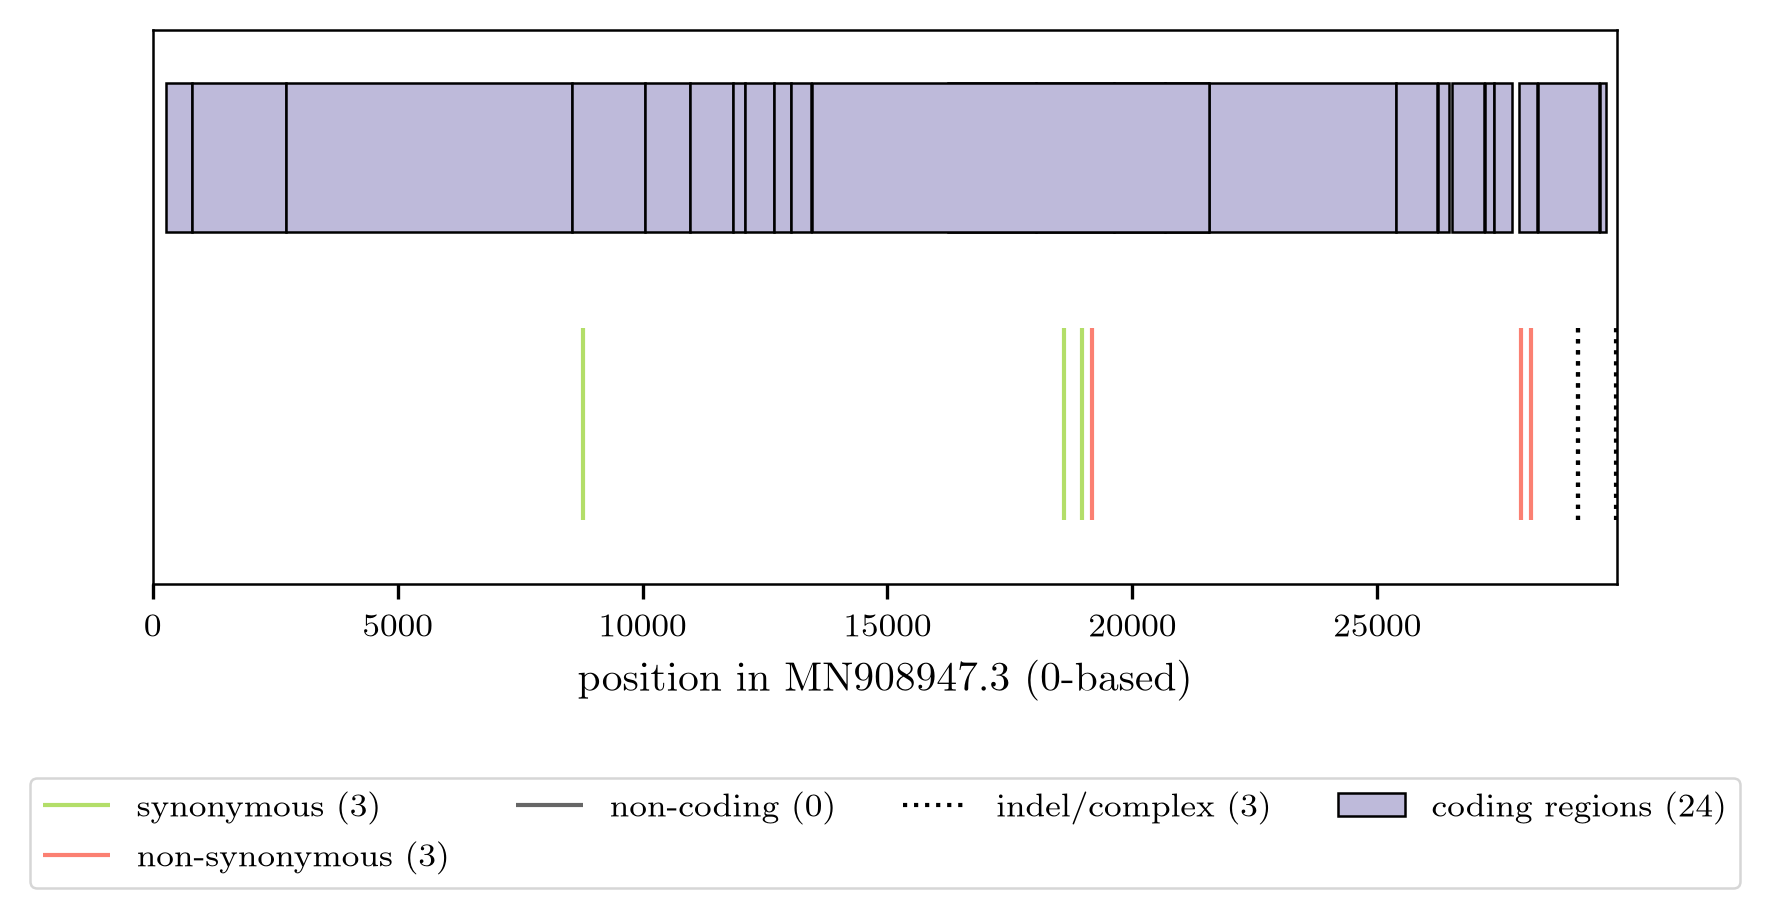
\includegraphics[width=0.98\linewidth]{fig_mutation_map}\par
      \fcap{Differences along MN908947.3; coding regions from backtracking.}
    \end{column}
    \begin{column}{0.32\textwidth}
      \small
      \begin{tabular}{@{}lr@{}}
        \toprule
        Wuhan length & 29\,903 \\
        Texas length & 29\,882 \\
        $|LCS|$ & \hl{29\,875} \\
        similarity & \hl{0.99906} \\
        substitutions & 6 \\
        \quad synonymous & 3 \\
        \quad non-synonymous & 3 \\
        indels & 3 \\
        Hirschberg time & 3.9 s \\
        DP table (not run) & 3.6 GB \\
        \bottomrule
      \end{tabular}
    \end{column}
  \end{columns}
  \note{The LCS counts symbols that can be kept in order in both genomes: 28 symbols of Wuhan and 7 of Texas have no partner. It ignores locality, which is why the gap analysis is needed to say where the differences are. Alignment took 3.9 s where the textbook table would need 3.6 GB.}
\end{frame}

% 6. results: the substitutions
\begin{frame}{The six substitutions: three silent, three change the protein}
  \begin{center}
    \footnotesize
    \begin{tabular}{rrcclcl}
\hline
Wuhan pos & Texas pos & base & region & codon & amino acid & effect \\
\hline
8782 & 8782 & C$\to$T & QHD43415\_4 & AGC$\to$AGT & S$\to$S & synonymous \\
18603 & 18603 & T$\to$C & QHD43415\_13 & CAT$\to$CAC & H$\to$H & synonymous \\
18975 & 18975 & T$\to$A & QHD43415\_13 & GTT$\to$GTA & V$\to$V & synonymous \\
19175 & 19175 & A$\to$C & QHD43415\_13 & GAT$\to$GCT & D$\to$A & non-synonymous \\
27925 & 27925 & C$\to$T & QHD43422 & ACA$\to$ATA & T$\to$I & non-synonymous \\
28144 & 28144 & T$\to$C & QHD43422 & TTA$\to$TCA & L$\to$S & non-synonymous \\
\hline
\end{tabular}
  \end{center}
  \smallskip
  \small
  \begin{itemize}
    \item The three indels sit after $29\,000$: a 21-nucleotide poly-A run missing from Texas (how far the read went, not a mutation), and an indel pair three positions apart that is really one more substitution, C$\to$T at $29\,095$. The LCS has no substitution operation, so an indel pair and a substitution can tie: the limit of an LCS as a diff.
    \item The last two rows fall outside the three gene files; they were classified only after backtracking located QHD43422.
  \end{itemize}
  \note{Gap argument if asked: consecutive matched pairs delimit a gap whose two sides share no symbol, so equal-length gaps are substitutions and one-sided gaps are indels. Codon effect: translate in both genomes with the standard code.}
\end{frame}

% 7. results: the frameshift
\begin{frame}{Backtracking found the ribosomal frameshift}
  \begin{columns}[c]
    \begin{column}{0.42\textwidth}
      \centering
      \small
      \begin{tabular}{@{}lrr@{}}
        \toprule
        protein & start & matched \\
        \midrule
        QHD43415\_10 & 13024 & 139/139 \\
        \hl{QHD43415\_11} & 13441 & \hl{9/932} \\
        QHD43415\_12 & 16236 & 601/601 \\
        \bottomrule
      \end{tabular}\\[0.4em]
      \fcap{Three of the 24 records, 0-based positions.}
    \end{column}
    \begin{column}{0.56\textwidth}
      \small
      \begin{itemize}
        \item 23 of 24 proteins located over their full length, a few dozen nodes each.
        \item The exception matches exactly 9 amino acids from $13\,441$, that is up to nucleotide $13\,468$: the ORF1a / ORF1b ribosomal frameshift, where the reading frame moves by one base.
        \item Translating ORF1ab in both frames finds 10 records whole in the first and 4 in the second, which validates the frames and the codon table.
        \item The search did not fail; it found a fact about the data.
      \end{itemize}
    \end{column}
  \end{columns}
  \note{Backtracking searches only the first k = 6 amino acids; the state is the set of genome positions still consistent, empty set prunes the subtree, survivors are verified by translating the whole protein forward.}
\end{frame}

% 8. comparison: time scaling
\begin{frame}{Running time against input size}
  \begin{columns}[c]
    \begin{column}{0.52\textwidth}
      \centering
      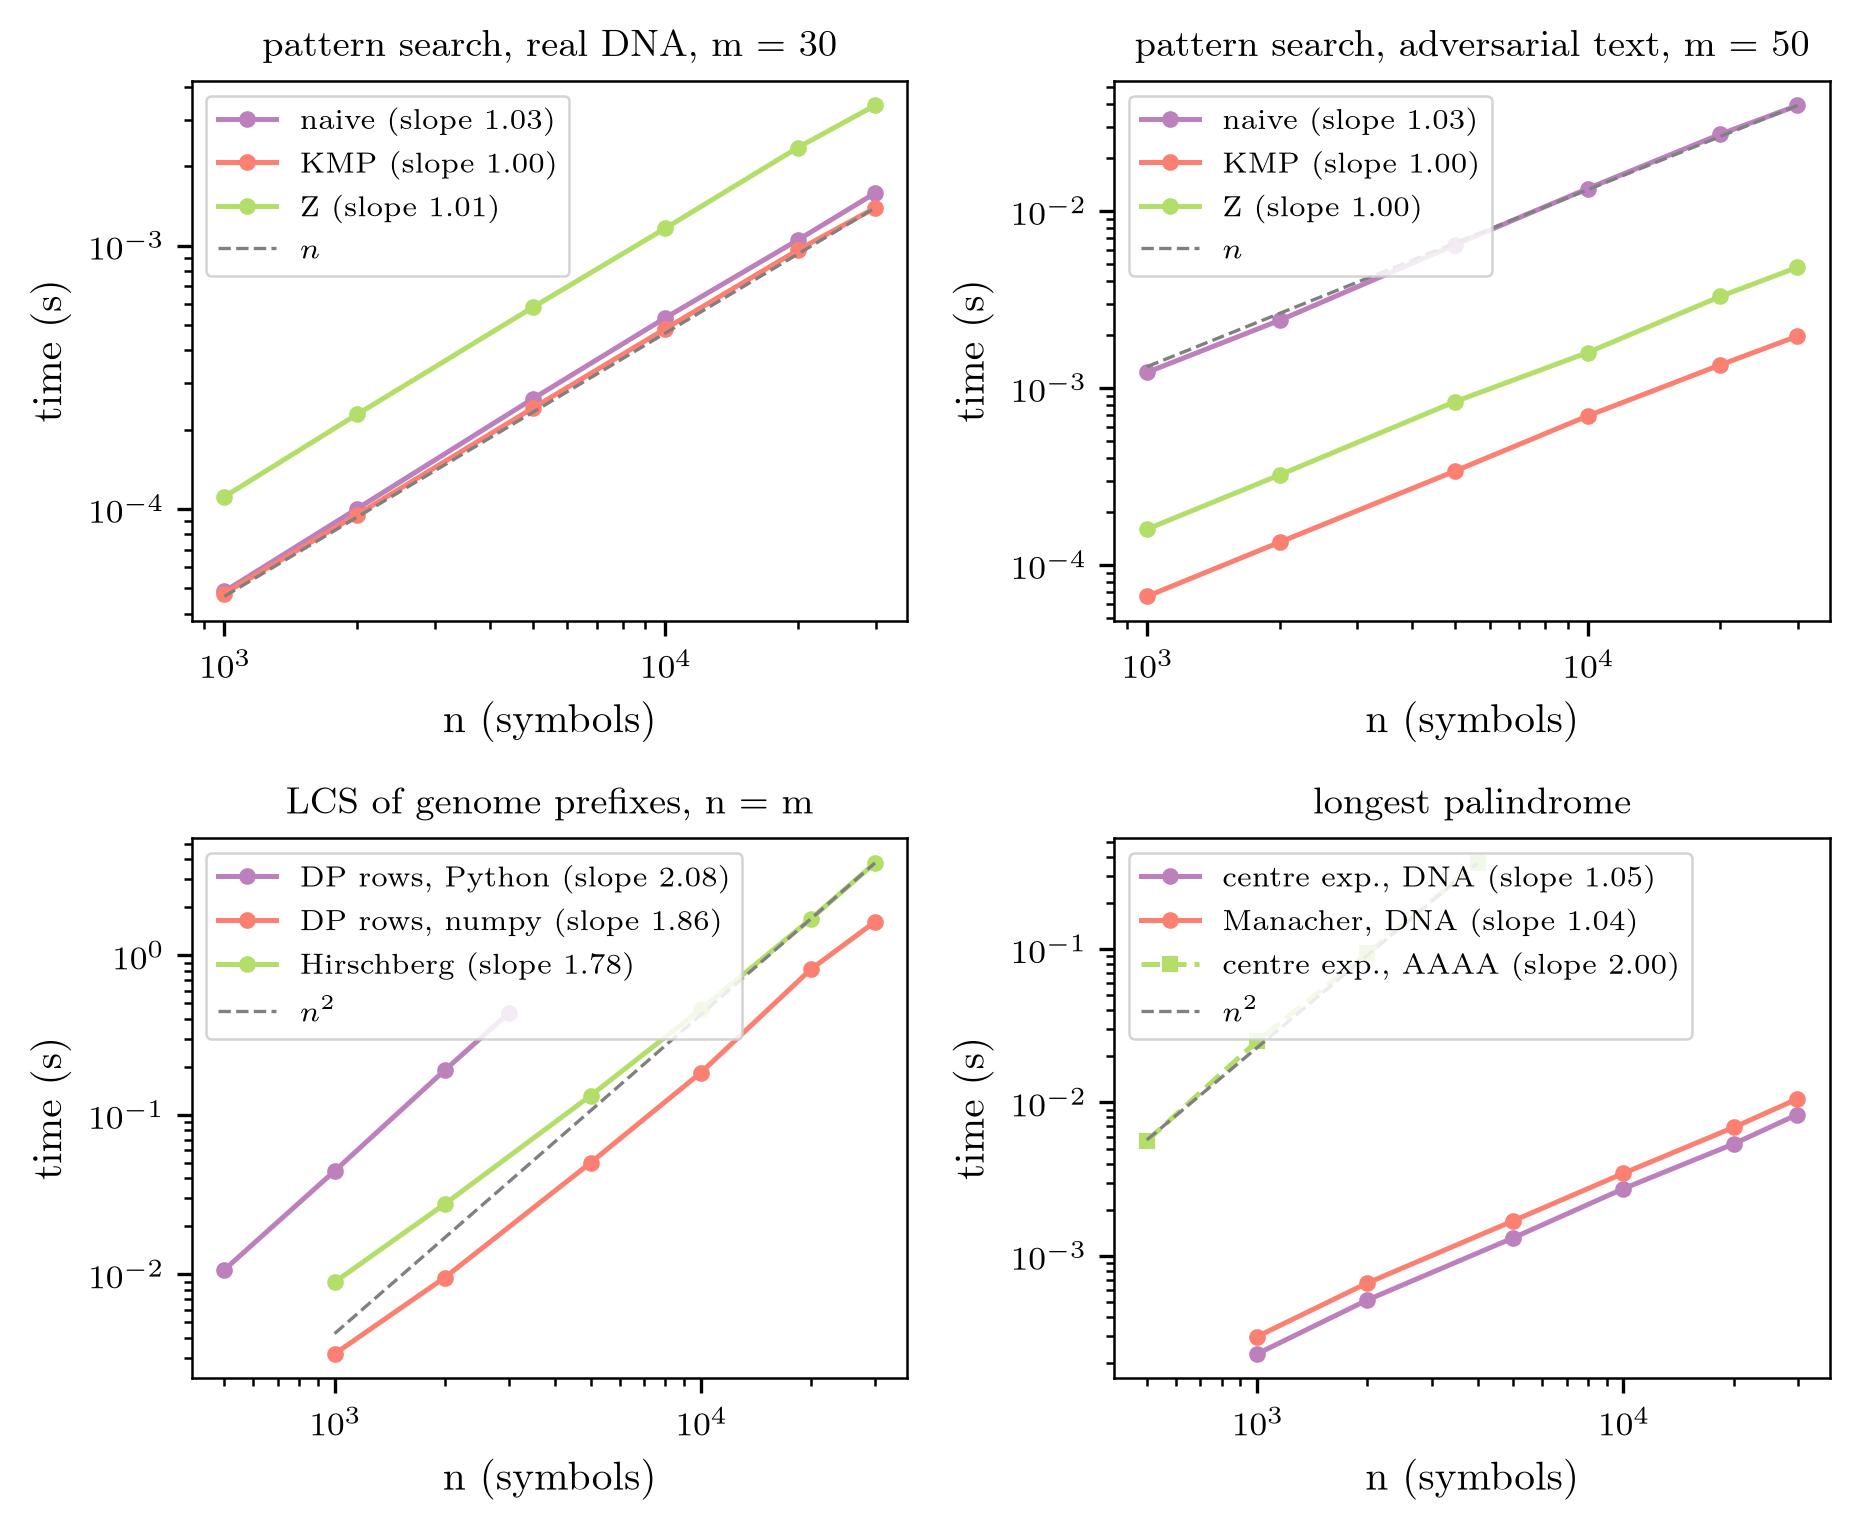
\includegraphics[height=0.74\textheight]{fig_time_scaling}\par
      \fcap{Log-log; dashed lines are the theoretical growth.}
    \end{column}
    \begin{column}{0.46\textwidth}
      \small
      \begin{itemize}
        \item \textbf{Search, real DNA:} all linear; naive is not slower because a mismatch ends most alignments after one or two comparisons.
        \item \textbf{Adversarial $A^n$:} naive keeps slope 1 but runs 20$\times$ slower than KMP, the factor $m = 50$.
        \item \textbf{LCS:} slope $\approx 2$ for all three; Hirschberg $\approx 2\times$ numpy rows, the $2nm$ bound; pure Python reaches only $n = 3\,000$ in the time numpy takes for the genomes.
        \item \textbf{Palindromes:} centre expansion linear on DNA, quadratic on $A^n$; Manacher linear on both.
      \end{itemize}
    \end{column}
  \end{columns}
  \note{The point to land: the log-log slopes reproduce the theoretical exponents, and the constants (numpy vs Python, 2nm vs nm) decide the actual run. Z is slower than KMP because it builds and stores an array of n + m + 1 values while KMP keeps one pointer.}
\end{frame}

% 9. comparison: search space
\begin{frame}{Search-space techniques against their exhaustive baselines}
  \begin{center}
    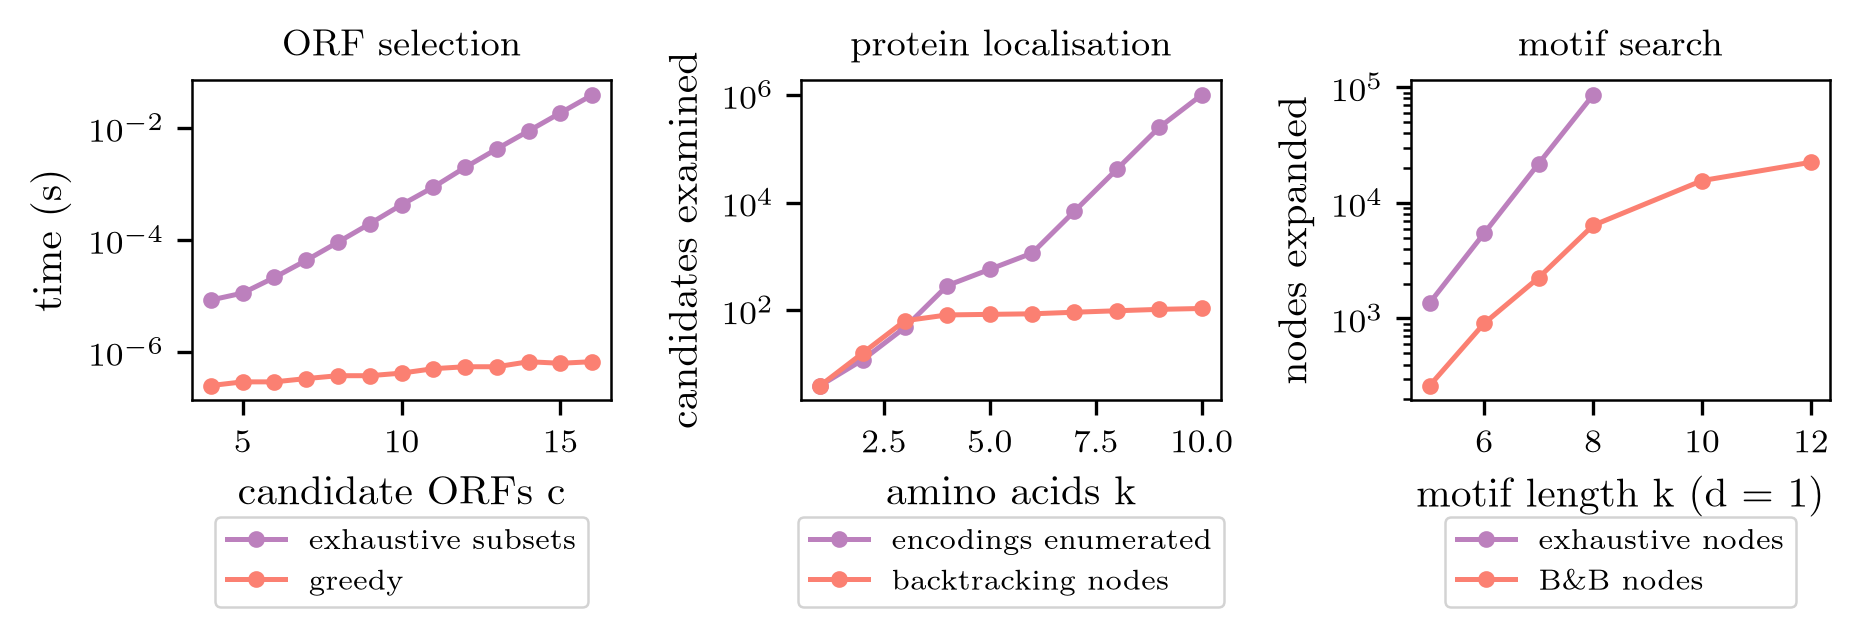
\includegraphics[width=0.78\textwidth]{fig_search_space}
  \end{center}
  \vspace{-0.6em}
  \small
  \begin{itemize}
    \item \textbf{Greedy:} exhaustive subsets double with every candidate ORF; greedy is flat.
    \item \textbf{Backtracking:} encodings grow with codon degeneracy, $10^6$ at $k = 10$; nodes stay near 100 because three amino acids pin one genome position.
    \item \textbf{Branch and bound:} same optimum as exhaustive search (TGTTGTTA, 75 hits) with 7\% of the nodes at $k = 8$; still runs at $k = 12$, where exhaustive search cannot.
  \end{itemize}
  \note{Caveat to say out loud: branch and bound saves nodes, not time. The bound, the number of alive positions, is loose at shallow depth, and that is where the filtering work happens.}
\end{frame}

% 10. conclusions
\begin{frame}{Which technique won, and why}
  \footnotesize
  \begin{columns}[T]
    \begin{column}{0.47\textwidth}
      \lead{Winner: divide and conquer over DP}
      \begin{itemize}
        \item Hirschberg turned an infeasible run into a feasible one: a 3.6 GB table became $O(n + m)$ rows and 3.9 s for two full genomes.
        \item Memory bound changed, time bound not: still $O(nm)$, about 2$\times$ the length-only rows, exactness never traded.
        \item Every other technique reached an answer brute force could also reach, given time; this one reached an answer brute force could not.
      \end{itemize}
    \end{column}
    \begin{column}{0.5\textwidth}
      \lead{Across techniques}
      \begin{itemize}
        \item \textbf{Scaled best:} linear string algorithms and greedy, slope $\approx 1$ on every input.
        \item \textbf{Cost most:} LCS at slope 2, and every exhaustive baseline: $2^c$, $6^k$, $4^k$.
        \item \textbf{Datasets flipped behaviour:} adversarial input flips naive vs KMP (20$\times$) and centre expansion vs Manacher (slope 1 to 2); the codon threshold flips greedy.
        \item \textbf{Pruning saves nodes, not time:} backtracking because the genome pins the prefix; branch and bound only as good as its bound.
      \end{itemize}
    \end{column}
  \end{columns}
  \vspace{0.1em}
  {\color{accent}\rule{\textwidth}{0.5pt}}\\[0.05em]
  \normalsize\textbf{Run the baseline.} Slopes reproduce the exponents, constants decide the run, and only the baseline says whether the clever algorithm was needed.
  \note{Close on the last line. If time allows, the one-line lesson per technique: DP exact but memory-bound; linear string algorithms justified by the worst case, not the average; greedy optimal only for the objective it is given; backtracking cheap because the constraint is strong; branch and bound limited by its bound; Manacher invisible on real data, visible under adversarial input.}
\end{frame}

\end{document}
